\documentclass[answers]{exam}
\usepackage{../../template}
\title{Problem Set 1}
\author{niceguy}
\begin{document}
\maketitle

\begin{questions}

\question{For the circuit shown below, find the voltage and current of each diode.}

\begin{figure}[h]
    \begin{center}
    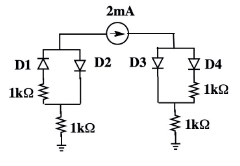
\includegraphics[width=0.3\textwidth]{q1.png}
    \end{center}
\end{figure}
    
\begin{parts}
    \part{Assume the diodes are ideal.}
    \part{Assume a 0.7V, constant voltage drop (CVD) diode model.}
    \part{Assume a "1mA diode" exponential diode model (i.e., that V=0.7V when I=1mA). Assume thermal voltage $V_T = 25\unit{mV}$.}
\end{parts}

\begin{solution}
    Assuming ideal diodes, we assume $D_3$ is on and $D_4$ is off. This is because either needs to be on according to KCL. But if $D_4$ is on, there is a voltage drop across the $1\unit{k\Omega}$ resistor, meaning there is a voltage drop across $D_3$, so $D_3$ has to be on regardless. But if it is on, there should be no voltage drop across $D_3$. If $D_4$ is on, there there is no voltage drop across the resistor, which is impossible. Hence $D_3$ is on and $D_4$ is off. \\
    Looking on the left hand side, $D_1$ has to be on as there is no other way for current to "enter" and reach 2mA.  Then voltage across $D_2$ has a negative bias, so $D_2$ is off. Hence \\
    \begin{center}
    \begin{tabular}{|c||c|c|}
        \hline
        Number/Measurement & Voltage (V) & Current (mA) \\
        \hline\hline
        1 & 0 & 2 \\
        \hline
        2 & -2 & 0 \\
        \hline
        3 & 0 & 2 \\
        \hline
        4 & 0 & 0 \\
        \hline
    \end{tabular}
    \end{center}
    With a 0.7V constant voltage drop, the same analysis applies, so $D_1$ and $D_3$ are on, and $D_2$ and $D_4$ are off. Then
    \begin{center}
    \begin{tabular}{|c||c|c|}
        \hline
        Number/Measurement & Voltage (V) & Current (mA) \\
        \hline\hline
        1 & 0.7 & 2 \\
        \hline
        2 & -2.7 & 0 \\
        \hline
        3 & 0.7 & 2 \\
        \hline
        4 & 0.7 & 0 \\
        \hline
    \end{tabular}
    \end{center}
    For the 1mA model, we use
    $$V_{D_1} - V_{D_2} = V_T\ln\left(\frac{I_{D_1}}{I_{D_2}}\right)$$
    Putting $I_1 = 2, I_2 = 1, V_2 = 0.7$, we get $V_1 = 0.717\unit{V}$, which is close to 0.7V as assumed in our previous model. On the other side, we have
    \begin{align}
        I_3 + I_4 &= 2 \\
        V_3 &= V_4 + I_4 \\
        V_T\ln\left(\frac{I_3}{I_4}\right) &= V_3 - V_4
    \end{align}
    One can use numeric methods to solve this.
\end{solution}

\question{For the circuit shown below, sketch the output waveform, $v_o(t)$ and find $v_o(t)$ at time $t=3\unit{ms}$. Assume the diode is ideal and the capacitor is initially discharged.}

\begin{figure}[h]
    \begin{center}
        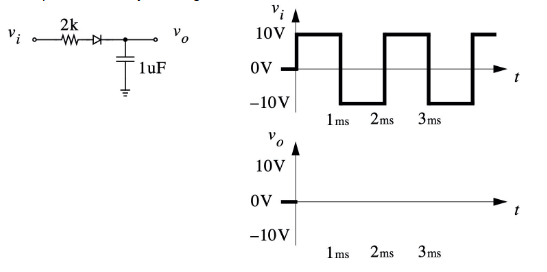
\includegraphics[width=0.5\textwidth]{q2.png}
    \end{center}
\end{figure}

\begin{solution}
    When voltage is positive, the diode behaves like a perfect conductor, so this becomes an RC circuit. When voltage is negative, the diode behaves like an open circuit. There is no current through the capacitor since there is no change in voltage. This is as if the RC circuit is paused. It resumes when voltage is positive again. Hence, for $t$ from 0 to 1 ms, it follows $v_o(t) = V_\infty\left(1 - e^{-t/\tau}\right)$. From 1 ms to 2 ms, it is constant and equal to $v_o(1)$. From 2 ms to 3 ms, it resumes and obeys $v_o(t) = V_\infty\left(1 - e^{-(t-1)/\tau}\right)$.
\end{solution}

\end{questions}

\end{document}
